\documentclass[a4paper, 11pt]{article}
\usepackage[utf8x]{inputenc}
\usepackage{graphics} % for pdf, bitmapped graphics files
\usepackage{graphicx} % for pdf, bitmapped graphics files
\usepackage[top=1in, bottom=1in, left=1in, right=1in]{geometry}
\usepackage{subfigure}
\usepackage{epsfig} % for postscript graphics files
\usepackage{mathptmx} % assumes new font selection scheme installed
\usepackage{amsmath} % assumes amsmath package installed
\usepackage{amssymb}  % assumes amsmath package installed
\usepackage[linesnumbered, vlined, ruled]{algorithm2e}
\usepackage{multicol}
\usepackage{placeins}
%%\usepackage[usenames, dvipsnames]{pstricks}
%%\usepackage{pst-grad}
%%\usepackage{pst-plot}
\usepackage{epstopdf}
\usepackage{bm}
\usepackage{url}
\usepackage{stfloats}
\usepackage{array}
\usepackage{booktabs}
\usepackage[table]{xcolor}
\usepackage[scaled=0.92]{helvet}


\usepackage{titlesec}
\usepackage{lastpage}
\usepackage{fancyheadings}
\usepackage{url}

\usepackage{tikz}
\usetikzlibrary{decorations.pathmorphing} % noisy shapes
\usetikzlibrary{fit}					% fitting shapes to coordinates
\usetikzlibrary{backgrounds}	% drawing the background after the foreground
\usetikzlibrary{shapes,arrows}
\usetikzlibrary{snakes,automata,petri}

\usepackage{hyperref}


%% Define a new 'leo' style for the package that will use a smaller font.
\makeatletter
\def\url@leostyle{%
  \@ifundefined{selectfont}{\def\UrlFont{\sf}}{\def\UrlFont{\small\ttfamily}}}
\makeatother
%% Now actually use the newly defined style.
\urlstyle{leo}

\pagestyle{fancy}
%\setlength{\footrulewidth}{0.4pt}
%\rhead{\bf A Generic Environment Model for better Human-Machine Communication}
\lfoot{Autonomous System Lab}
\cfoot{Ming Liu}
\rfoot{\thepage}
%
\newcommand{\mat}[2][rrrrrrrrrrrrrrrrrrrrrrrrrrrrrrrrrrrrrrrrrrrrrrrrrrr]{\left(
  \begin{array}{#1}
    #2 \\
  \end{array}
\right)}
\newcommand{\vect}[1]{\boldsymbol{#1}}
\newcommand{\HRule}{\rule{\linewidth}{0.5mm}}
\renewcommand{\rmdefault}{phv}

\title{\centering \LARGE \bf  Quick Guide to Tensor Voting using GPU (CUDA)}
\date{\today}
\author{Ming LIU \\  liu.ming.prc@gmail.com}

\titleformat{\section}[block]
{\normalfont\sffamily}
{\bf\thesection}{.5em}{\bfseries}

\titleformat{\subsection}[block]
{\normalsize\sffamily}
{\bf\thesubsection}{.5em}{\bfseries}

\titleformat{\subsubsection}[block]
{\normalsize\itshape}
{\thesubsubsection}{.5em}{\itshape}

\begin{document}

\maketitle

This document is a \textbf{very brief} introduction to the usage of the GPU library for 3D tensor voting. So don't hesitate to ask me for further details and help if you need.

\section{Pre-requirement for installation}

\subsection{CUDA and NVIDIA}
I think the main issue for most users maybe the installation of CUDA. Other than that, everything should be OK.
If you have problem in compilation the .cu files, even with cuda >3.0 installed, it means that your hardware may not compatible.
Update your NVIDIA driver to the latest always helps.


\textbf{Hint:}
  \begin{itemize}
  \item 
{\tt \$ nvcc --version} \\
to check the CUDA SDK version.

  \item 
it is a pity that the {\tt gpgpu} ros package is not updating anymore. In general, the official SDK from NVIDIA is enough.

{\tt https://developer.nvidia.com/cuda-downloads}
  \end{itemize}

\subsection{Other dependent packages}
The code is based on ETH-ASL libpointmatcher and libpointmatcher-ros library:

If you checked out the latest nifti-mapping ros-stack, it should be ok. Otherwise, get it from GitHub:

{\tt https://github.com/ethz-asl}

\section{Quick Tutorial after compilation}
\begin{enumerate}
\item ``rosmake'' in tensorvoting package\\
Usually it should work if the CUDA SDK is configured. Error may occur if the libpointmatcher is not properly installed.
\item You will get two executables in bin/ : {\tt demo\_dense\_gpu} and {\tt demo\_sparse\_gpu}.
They are corresponding to the concept of dense voting and sparse voting respectively \cite{mordohai2006tensor,schuster2004segmentation}.
To try these two samples, the launch files in launch/ can be used.
\item \textit{sparse voting}:\\
    use {\tt demo\_sparse\_gpu.launch}. It will load (by default) the dataset data/planes4.vtk then extract sparse tensor from it.
    (.vtk files are supported by paraview. please refer to the next section)
It will keep doing that in loop, unless a ctrl-c kill to the processes.
An rviz will be opened and showing the sparse information. You may see something like the following:\\
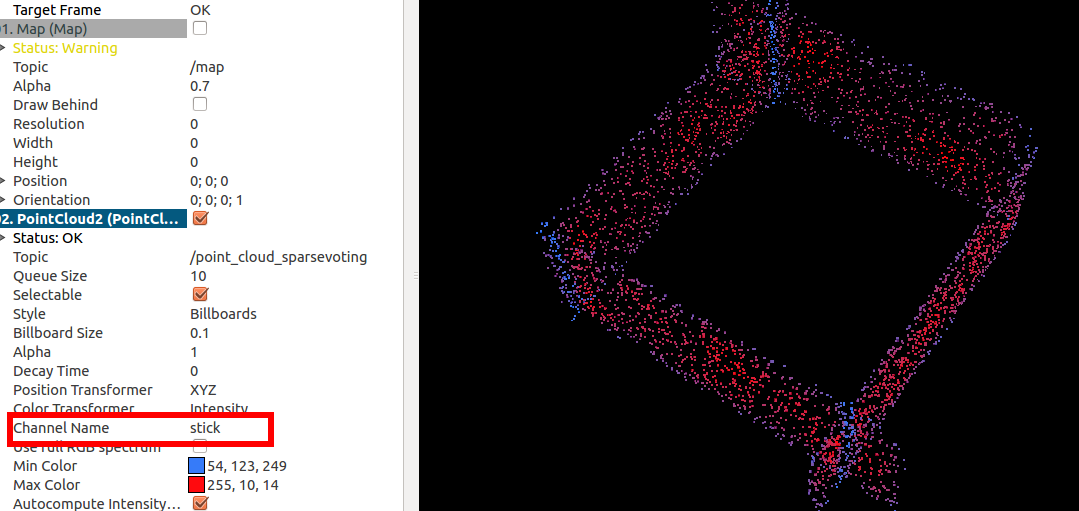
\includegraphics[width=\textwidth]{sparse}.

Note that, you can change the channel on the left (highlighted by red rectangle) to switch the representation (stick saliency, plate, ball, x, y, z etc.) 
In this sample, you see the red-ish color show the magnitude to be considered as planes (stick saliency).

\item \textit{dense voting}:\\
similar thing. However, it is not recommended to use rviz to show the result, as explained in the next section.

\item The parameters can be modified from the launch files to tune different datasets. e.g. {\tt sigma} for the kernel size.

\end{enumerate}


\section{vtk files and dense voting result inspection}
We mainly use paraview ({\tt apt-get install paraview}) to inspect the result of point-clouds.
This GPU implementation allows to save .vtk files for further review. It can be turned on by setting the parameter in .launch {\tt savevtk}.
The following examples show how they may look like in paraview (stick component, plate component, normal estimation):\\
{
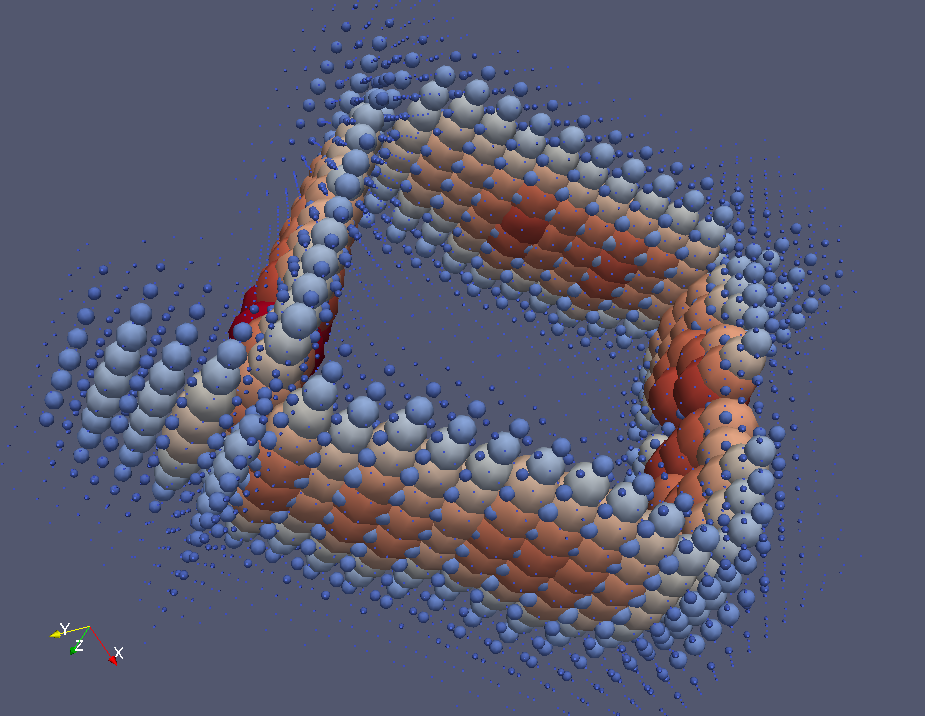
\includegraphics[width=0.7\textwidth]{pv_stick}\\
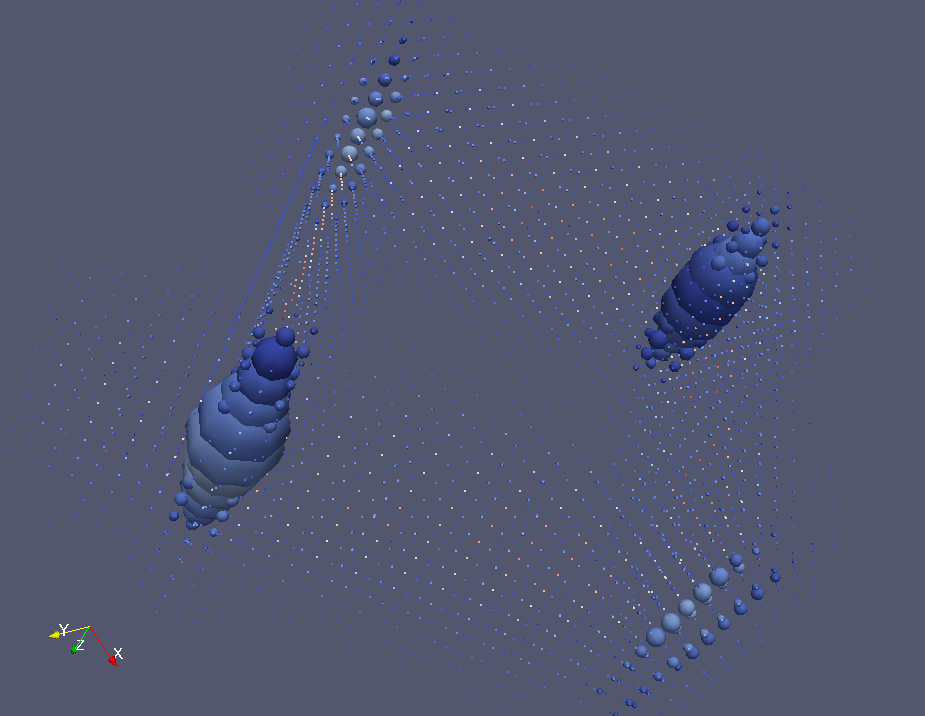
\includegraphics[width=0.7\textwidth]{pv_plate}\\
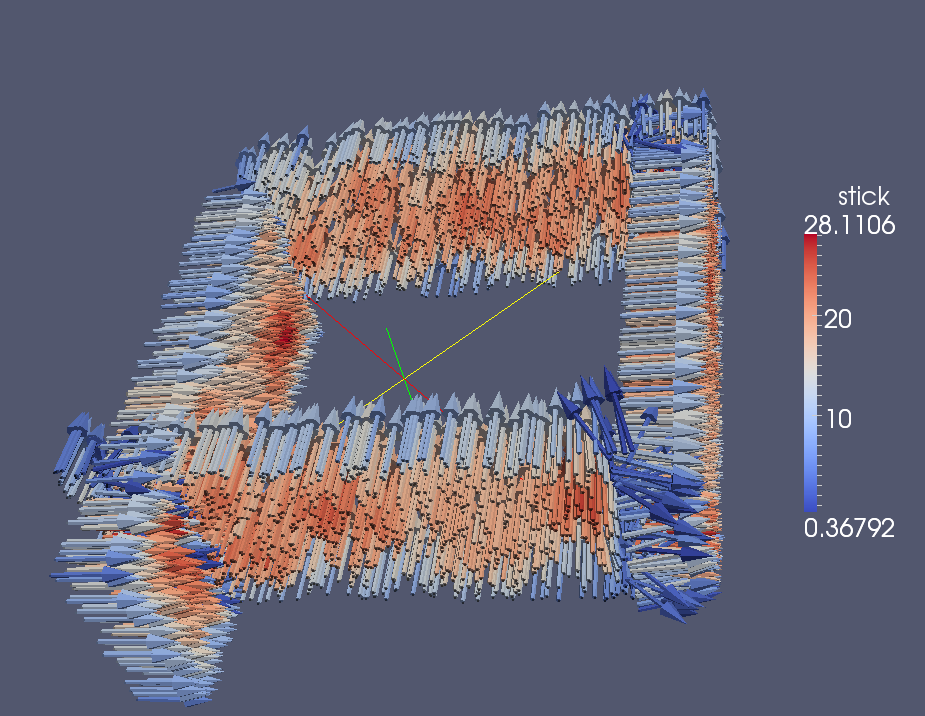
\includegraphics[width=0.7\textwidth]{pv_normal}
}



For further information, please refer to: \cite{liu12robio}

BTW: if you need an omnidirectional camera image dataset with vicon ground truth (used for visual homing, visual odometry etc), please visit my website:
http://www.asl.ethz.ch/people/lium/personal


\bibliographystyle{plain}
\bibliography{new_lib}

\end{document}
